	\documentclass[12 pt]{article}

	\usepackage[frenchb]{babel}
	\usepackage[utf8]{inputenc}  
	\usepackage[T1]{fontenc}
	\usepackage{amssymb}
	\usepackage[mathscr]{euscript}
	\usepackage{stmaryrd}
	\usepackage{amsmath}
	\usepackage{tikz}
	\usepackage[all,cmtip]{xy}
	\usepackage{amsthm}
	\usepackage{varioref}
	\usepackage{geometry}
	\geometry{a4paper}
	\usepackage{lmodern}
	\usepackage{hyperref}
	\usepackage{array}
	 \usepackage{fancyhdr}
	 \usepackage{eurosym}
\usepackage{float}
	\pagestyle{fancy}
	\theoremstyle{plain}
	\fancyfoot[C]{\empty} 
	\fancyhead[L]{Exercices}
	\fancyhead[R]{2021-2022}
	\newcounter{n}
	\numberwithin{n}{section}
	\newtheorem{df}[n]{Définition}
	\newtheorem{theo}{Théorème}
	\labelformat{theo}{théorème}
    \newtheorem{rmq}[n]{Remarque}
	\labelformat{rmq}{remarque~#1}
	\newtheorem{cor}[n]{Corollaire}
	\newtheorem{lm}{Lemme}
	\labelformat{lm}{lemme~#1}
	\newtheorem{hyp}[n]{Hypothèse}
	\newtheorem{nt}[n]{Notation}

	\renewcommand\epsilon{\varepsilon}
	\renewcommand\phi{\varphi}
	\newcommand\R{\mathbb{R}}
	\newcommand\s{\mathbb{S}}
	
	
	
	\title{Exercices Chapitre 5}
	\date{}
	\begin{document}

\begin{center}{\Large Chapitre 7 - Calcul littéral - Révisions}\\ 
 \end{center}

\section{Exercice 1}

Évaluer les expressions suivantes : \begin{itemize}
\item[a) ]  $2\times x +3$ en $x=1$, $x=2$ et $x=-6$.   
\item[b) ]  $2\times x +y$ en $x=1$ et $y=5$, puis en $x=-2$ et $y=4$.   
\item[c) ]  $x \times y - (x-1) \times (y-1) $ en $x=1$ et $y=3$, puis en $x=2$ et $y=9$. 
\end{itemize}
\section{Exercice 2}

Exprimer les grandeurs suivantes par une expression littérale. 

\begin{itemize}
\item[a) ] Le double de la somme de $x$ et $y$.
\item[b) ] Le quart de la différence de $1$ et de $x$. 
\item[c) ] Le quotient de la somme de $x$ et de $1$ par $y$. 
\item[d) ] La somme du quotient de $3$ par $x$ et du produit de $y$ et $4$.
\end{itemize}

\section{Exercice 3}

Exprimer les propriétés suivantes par des égalités :

\begin{itemize}
\item[a) ] La somme de $x$ et de $4$ est égale à la différence de $y$ et $5$. 
\item[b)] Le produit de $3$ et $a$ est égal au quotient de $a$ par $5$. 
\item[c)] La somme de $a$ et $b$ est égale à leur produit. 
\end{itemize}



\section{Exercice 4}

Le prix de cinq cahiers est de $19,40$\euro . 

1) On note $c$ le prix d'un seul cahier. Écrire une formule donnant le prix de cinq cahiers. 

2) En déduire une égalité vérifiée par $c$. 

3) Trouver la valeur de $c$ vérifiant cette égalité. 



\section{Exercice 5}

Un stylo et une cartouche ensemble coûtent $2$\euro{}. 
Le stylo coûte $1$ \euro{} de plus que la cartouche.

1) On note $c$ le prix de la cartouche. Exprimer le prix du stylo en fonction de $c$. 

2) Exprimer le prix d'un stylo et d'une cartouche en fonction de $c$. En déduire une égalité vérifiée par $c$. 

3) Trouver $c$. En déduire le prix du stylo et celui de la cartouche.  

\section{Exercice 6}

Le prix de cinq cahiers et de trois stylos est de $19,40$ \euro{} . 

1) On note $c$ le prix d'un seul cahier et $s$ celui d'un stylo. Écrire une formule donnant le prix de cinq cahiers et de trois stylos en fonction de $c$ et $s$. 

2) En déduire une égalité vérifiée par $c$ et $s$. 

3) Vérifier si les prix suivants sont cohérents avec l'énoncé : 

a) $c= 2$ \euro{}, $s= 1,5$ \euro{}

b) $c = 1,90$ \euro{}, $s= 3, 30$ \euro{}.

4) a)Si un cahier coûte $1$\euro{}, combien coûtera un stylo ? 

b) Si un stylo coûte $2$\euro{}, combien coûtera un cahier ? 
\newpage
\section{Exercice 7}

On construit une suite de segments de la manière suivante. \begin{itemize}
\item[A] On commence avec un segment de longueur $1$. 
\item[B] On supprime le tiers central de ce segment, et on le remplace par deux segments de même longueur.
\item[C] On recommence l'étape précédente avec chacun des segments de la figure obtenue
\item[D] On recommence l'étape 2. avec chacun des segments de la nouvelle figure. 
\item etc. 
\end{itemize}
\begin{figure}[H]\center
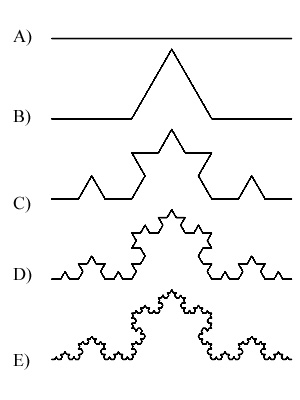
\includegraphics[scale=.75]{Droite_koch}
\end{figure}

1) Combien de segments y a-t-il sur la figure à l'étape $B$ ? à l'étape $C$ ? 

2) Peut-on trouver le nombre de segments à l'étape $D$ (sans compter directement sur la figure) ?

3) Donner une formule exprimant le nombre de segments sur la figure à l'étape $F$ ? (On ne demande pas de calculer le résultat de cette formule.) 

4) [Plus dur] Mêmes questions concernant la longueur totale des segments à chaque étape. 
	\end{document}
